\documentclass{article}
\usepackage{amsmath,amssymb}
\usepackage{tikz}
\usetikzlibrary{arrows.meta,positioning,calc,shapes.geometric}
\pagestyle{empty}
\begin{document}
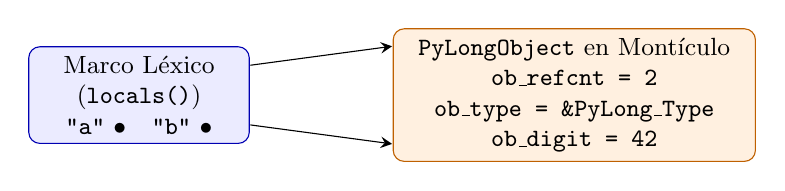
\begin{tikzpicture}
\tikzset{node distance=1.8cm, >=stealth, thick, font=\small}
\node[draw=blue!70!black, fill=blue!8, rounded corners, minimum width=2.8cm, minimum height=1.2cm, align=center] (ns) {Marco Léxico\\(\texttt{locals()})\\\texttt{"a"} $\bullet$\quad \texttt{"b"} $\bullet$};
\node[draw=orange!75!black, fill=orange!12, rounded corners, minimum width=4.6cm, minimum height=1.4cm, align=center, right=1.8cm of ns] (obj) {\texttt{PyLongObject} en Montículo\\\texttt{ob\_refcnt = 2}\\\texttt{ob\_type = \&PyLong\_Type}\\\texttt{ob\_digit = 42}};
\draw[->] (ns.15) -- (obj.165);
\draw[->] (ns.345) -- (obj.195);
\end{tikzpicture}
\end{document}
